\documentclass{beamer}
%[aspectratio=169]   \usepackage[czech]{babel}
\usepackage{apo-lecture}
\usepackage{pdfpages}
\usepackage{pdfcomment}
\usepackage{listings}
\usepackage{array,multirow}

\subtitle{Lekce 04. Central Processing Unit (CPU)}
\author{Pavel Píša\\ \small\texttt{pisa@fel.cvut.cz}}
\begin{document}

\maketitle

\section{Simulátor}

\begin{frame}
\frametitle{QtMips and QtRVSim – Origin and Development}

\begin{itemize}
\item MipsIt used in past for Computer Architecture course at the Czech Technical University in Prague, Faculty of Electrical Engineering
\item Diploma theses of Karel Kočí mentored by Pavel Píša
Graphical CPU Simulator with Cache Visualization
https://dspace.cvut.cz/bitstream/handle/10467/76764/F3-DP-2018-Koci-Karel-diploma.pdf
\item Switch to QtMips in the 2019 summer semester
\item Fixes, extension and partial internals redesign by Pavel Píša
\item Switch to RISC-V architecture in 2022. Main work by Jakub Dupák 2021
Graphical RISC-V Architecture Simulator - Memory Model and Project Management
\item https://dspace.cvut.cz/bitstream/handle/10467/94446/F3-BP-2021-Dupak-Jakub-thesis.pdf

\item Alternatives:
\begin{itemize}
 \item RARS: IDE with detailed help and hints
 https://github.com/TheThirdOne/rars
 \item EduMIPS64: 1x fixed and 3x FP pipelines
 https://www.edumips.org/
\end{itemize}
\end{itemize}

\end{frame}


\begin{frame}
\frametitle{QtRVSim - Download}
\begin{itemize}
\item Windows, Linux, Mac
https://github.com/cvut/qtrvsim/releases
\item  Ubuntu
https://launchpad.net/~qtrvsimteam/+archive/ubuntu/ppa
\item Suse, Fedora and Debian
https://software.opensuse.org/download.html?project=home%3Ajdupak&package=qtrvsim
\item Suse Factory
TBD
\item Online version
https://dev.jakubdupak.com/qtrvsim/
\item LinuxDays 2019 QtMips talk – Record of Interactive Session
https://youtu.be/fhcdYtpFsyw
https://pretalx.linuxdays.cz/2019/talk/EAYAGG/
\end{itemize}
\end{frame}

\begin{frame}
\frametitle{John von Neumann}
\begin{center}
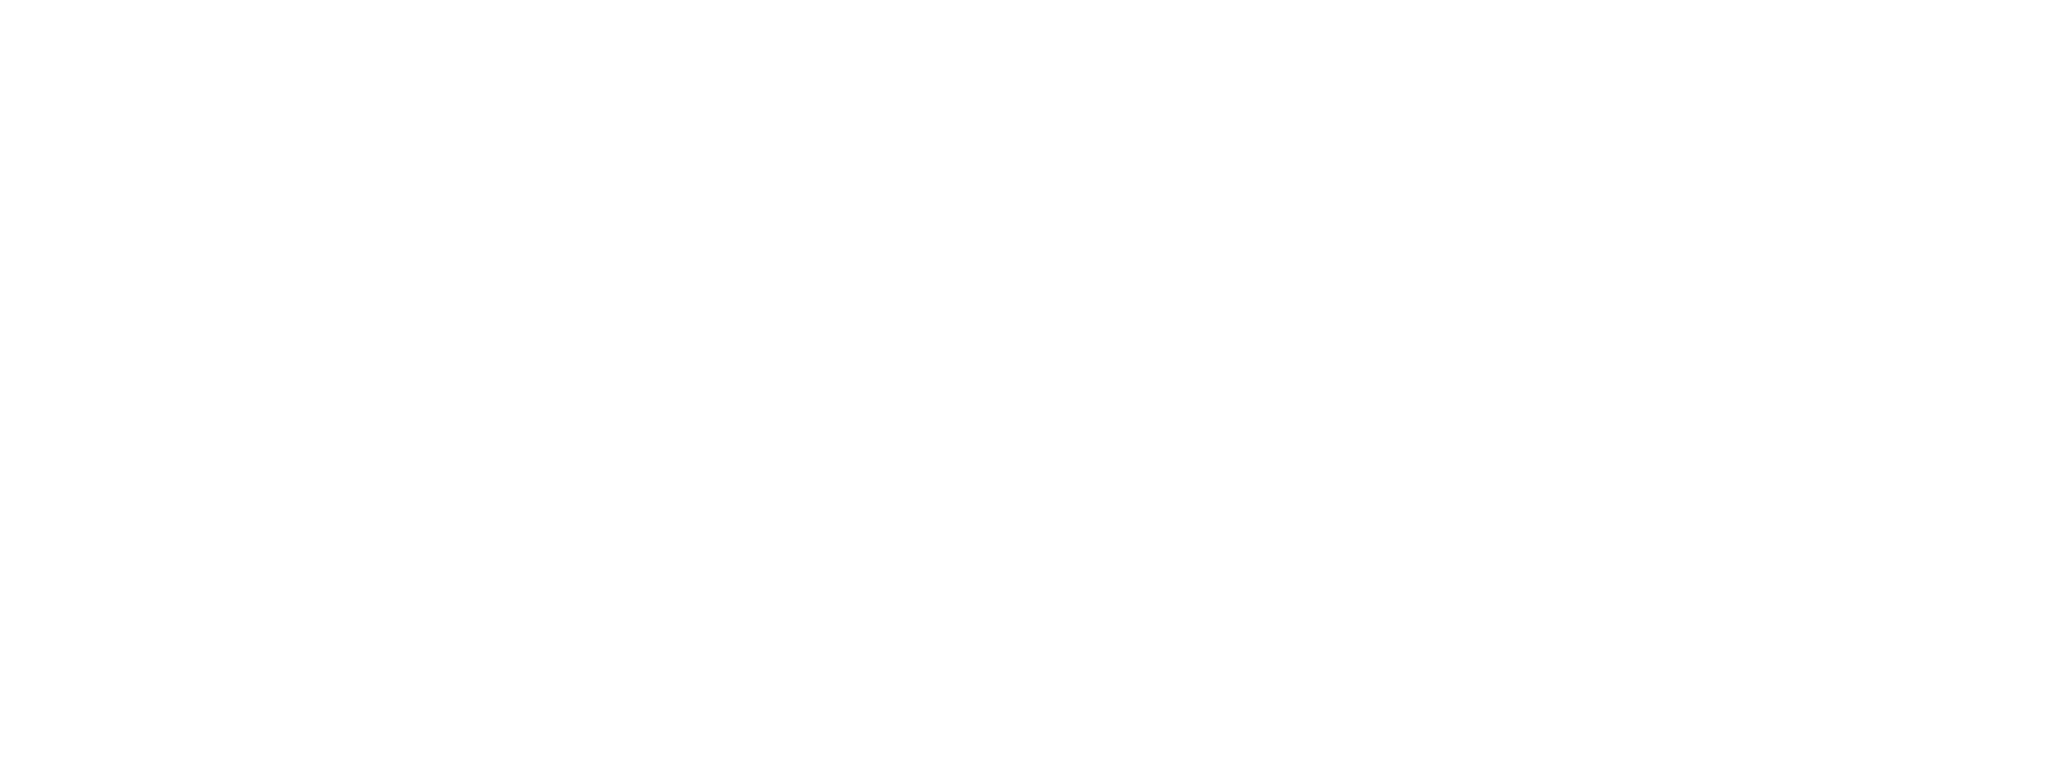
\includegraphics[width=0.65\textwidth]{cpu-vonNeumann.pdf}
\hfill
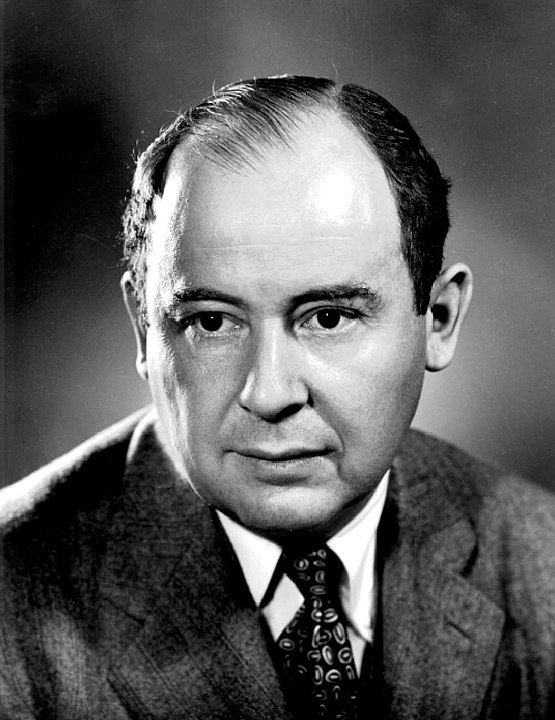
\includegraphics[width=0.2\textwidth]{fig/vonNeumann.png}
\end{center}
\begin{itemize}
\item 5 functional units – control unit, arithmetic logic unit, memory, input (devices), output (devices)
\item An computer architecture should be independent of solved problems. It has to provide mechanism to load program into memory. The program controls what the computer does with data, which problem it solves.
\item Programs and results/data are stored in the same memory. That memory consists of a cells of same size and these cells are sequentially numbered (address).
\item The instruction which should be executed next, is stored in the cell exactly after the cell where preceding instruction is stored (exceptions branching etc. ). 
\item The instruction set consists of arithmetics, logic, data movement, jump/branch and special/control instructions.
\end{itemize}
\end{frame}


\begin{frame}
\frametitle{Computer based on von Neumann's concept}

\begin{itemize}
\item Procesor/microprocessor
\begin{itemize}
\item Control unit
\item ALU
\end{itemize}
\item Memory - von Neumann architecture uses common memory, whereas Harvard architecture uses separate program and data memories
\item Input/output subsystem
\begin{itemize}
\item Input
\item Output
\end{itemize}
\end{itemize}
The control unit is responsible for control of the operation processing and sequencing. It consists of:
\begin{itemize}
\item registers – they hold intermediate and programmer visible state
\item control logic circuits which represents core of the control unit (CU)
\end{itemize}
\end{frame}


\begin{frame}
\frametitle{The most important registers of the control unit}
\begin{itemize}
\item PC (Program Counter)
holds address of a recent or next instruction to be processed
\item IR (Instruction Register)
holds the machine instruction read from memory
\item Another usually present registers
\begin{itemize}
\item General purpose registers (GPRs)
may be divided to address and data or (partially) specialized registers
\item SP (Stack Pointer) – points to the top of the stack; (The stack is usually used to store local variables and subroutine return addresses)
\item PSW (Program Status Word)
\item IM (Interrupt Mask)
\item Optional Floating point (FPRs) and vector/multimedia regs.
\end{itemize}
\end{itemize}
\end{frame}

\begin{frame}
\frametitle{The main instruction cycle of the CPU}
FLAGS registr 
\begin{enumerate}
  \item Initial setup/reset – set initial PC value, PSW, etc.
  \item Read the instruction from the memory
  \begin{itemize}
    \item PC → to the address bus
    \item Read the memory contents (machine instruction) and transfer it to the IR
    \item PC+l → PC, where l is length of the instruction
  \end{itemize}
  \item Decode operation code (opcode)
  \item Execute the operation
  \begin{itemize}
    \item compute effective address, select registers, read operands, pass them  through ALU and store result
  \end{itemize}
  \item Check for exceptions/interrupts (and service them)
  \item Repeat from the step 2
\end{enumerate}
\end{frame}


\begin{frame}[fragile]
\frametitle{Compilation: C  Assembler  Machine Code}

\begin{columns}
\begin{column}{0.3\textwidth}
\begin{lstlisting}[language={C},columns=flexible]
/* ffs as log2(x)*/
int x = 157;
int y = -1;
 
while(x != 0) {
  x = x / 2;
  y = y + 1;
}
\end{lstlisting}
\end{column}

\begin{column}{0.4\textwidth}  
\begin{lstlisting}[language={C},columns=flexible]
_start:
  addi a0, zero, 157  // int x = 157;
  addi t1, zero, -1   // int y = 0;
  beq a0, zero, done  // while(x != 0) {
loop:
  srli a0, a0, 1      //   x = x / 2;
  addi t1, t1, 1      //   y = y + 1;
  bne a0, zero, loop  //}
done:
  addi a0, t1, 0
\end{lstlisting}
\end{column}

\begin{column}{0.3\textwidth}  
\begin{lstlisting}[language={C},columns=flexible]
0x00000200  09d00513
0x00000204  fff00313
0x00000208  00050863
0x0000020c  00155513
0x00000210  00130313
0x00000214  fe051ce3
0x00000218  00030513
0x0000021c  00100073
\end{lstlisting}
\end{column}

\end{columns}

\end{frame}


\begin{frame}
\frametitle{Instruction Encoding Constrains}
\begin{itemize}
\item Encode 256 combinations in 8-bits
\item Opcode and address to directly operate on megabytes of ram does not fit
\item Use some limited number of fast accessible registers or use stack concept
\item 8 registers, 3 bits to encode, for two operand operations (a += b, mem[a] = b), 6 bits to select registers→only 4 operations in total
\item 16 bit (65536), 16 registers, 256 two operands or 16 three operands (4 + 3 * 4 bits)
\item 32 bit, 32 registers, three operands (17 + 3 * 5)
\item But immediate for arithmetic and address usually required (CISC followup words, RISC uses limited ranges and some other mechanism) 
\end{itemize}
\end{frame}


\begin{frame}[shrink=5]
\frametitle{RISC-V -- Instruction Length Encoding}

\begin{tabular}{r l}
  \begin{tabular}{|c|}\hline
  \texttt{xxxxxxxxxxxxxxaa}\\ \hline
  \end{tabular} & 16-bit (aa \neq 11)\\
   &  \\
   \begin{tabular}{|c|c|}\hline
  \texttt{xxxxxxxxxxxxxxxx} & \texttt{xxxxxxxxxxxbbb11}\\ \hline
  \end{tabular} & 32-bit (bbb \neq 111)\\
%\cline{2-3}
&  &  &  \\
Address:&  &  &  \\
base+4 & base+2 & base &  \\
\end{tabular}

\end{frame}


\begin{frame}
\frametitle{RISC-V Processor Registers}
\begin{tabular}{l l l l}
Register & ABI Name & Description & Saver \\
x0 & zero & Hard-wired zero &  \\
x1 & ra & Return address & Caller \\
x2 & sp & Stack pointer &  Callee\\
x3 & gp & Global pointer &  \\
x4 & tp & Thread pointer &  \\
x5-7 & t0--2 & Temporaries &  \\
x8 & s0/fp & Saved register/frame pointer & Callee \\
x9 & s1 & Saved register &  Callee \\
x10--11 & a0--2 & Function arguments/return values &  Caller \\
x12--17 & a2--7 & Function arguments & Caller \\
x18--27 & s2--11 & Saved registers & Callee \\
x28--31 & t3--6 & Temporaries &  \\
pc & pc & Program Counter &  \\
f0-31 &  & Floating point &  \\
\end{tabular}
\end{frame}



\begin{frame}
\frametitle{Hardware realization of basic (main) CPU cycle}

\end{frame}



\begin{frame}
\frametitle{Single cycle CPU – implementation of the load instruction}

\end{frame}

\end{document}

